\chapter{Описание архитектуры имитатора}\label{ch:ch2}

\begin{center}
    \begin{figure}[hb]
        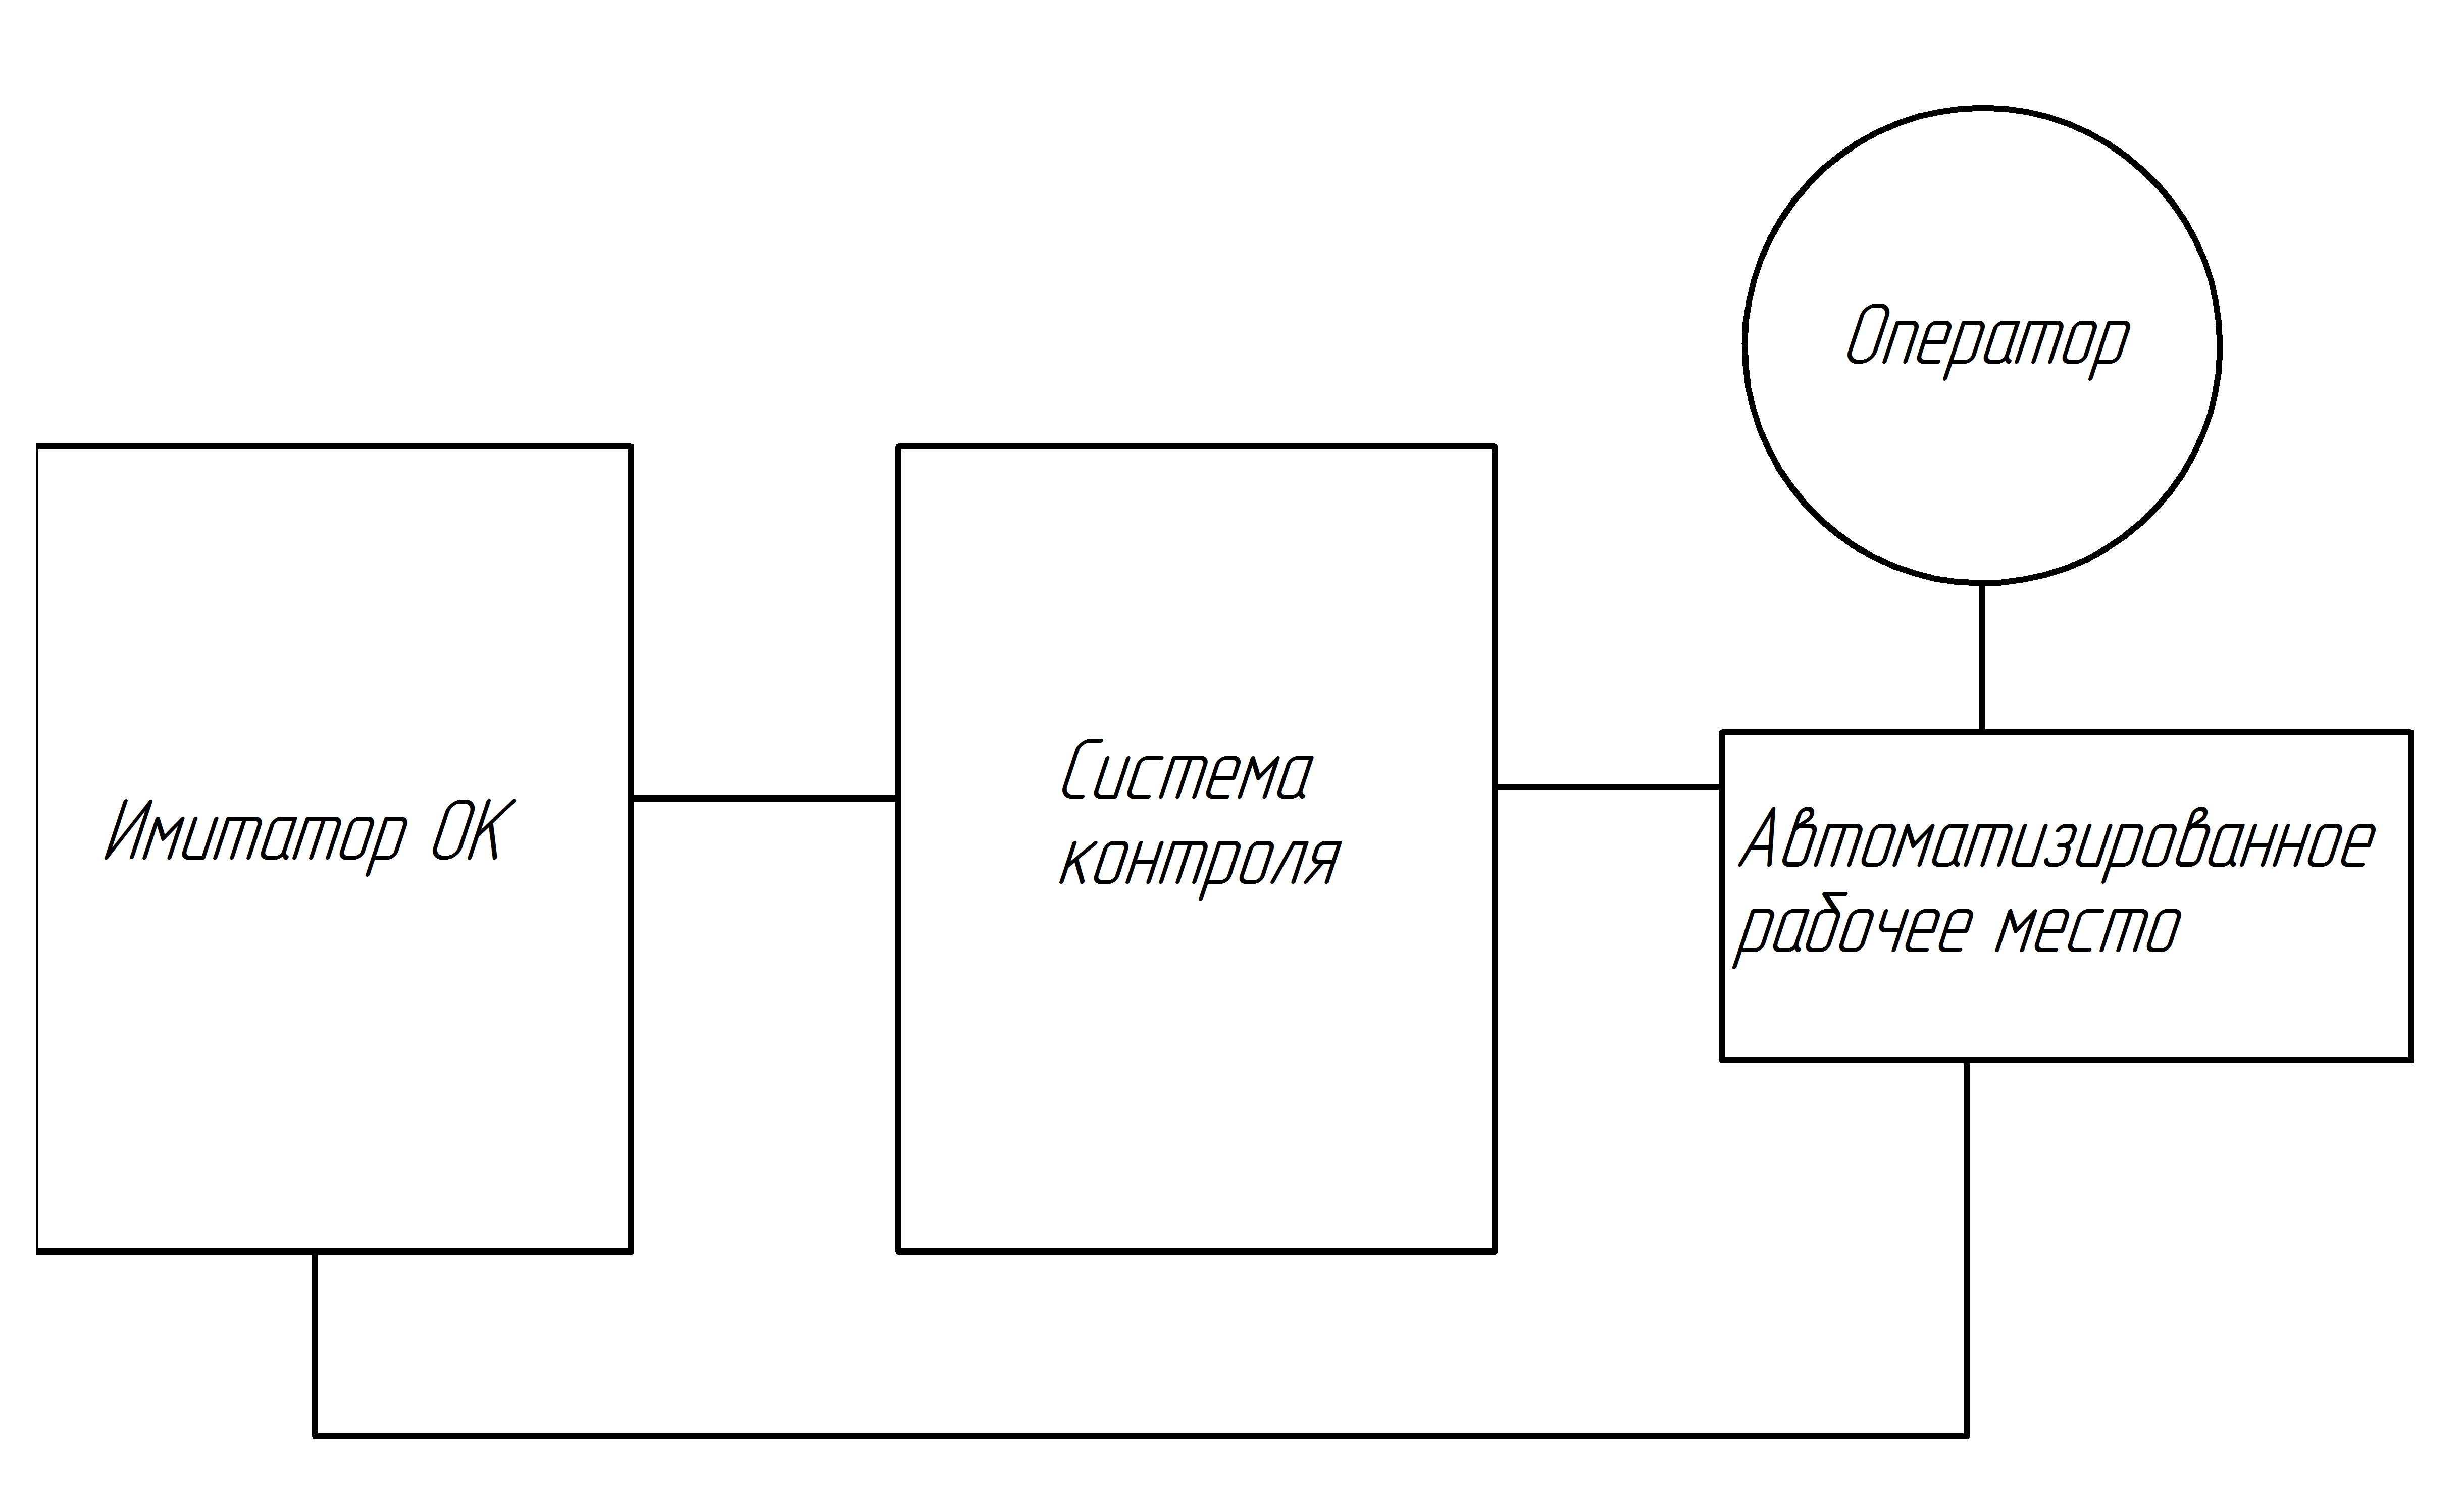
\includegraphics[width=.8\textwidth]{scheme.png}
        \caption{Структура программно-технологического комплекса}\label{fig:asc_schema}
    \end{figure}
\end{center}
    


\section{Распределение ролей}

На стороне СК создается экземпляр клиента сети modbus,
имитатор представляет сервер (см. главу \ref{ch:ch2}).





\section{Конфигурационный файл}\label{sec:ch2/sec1}

Общее пространство данных modbus у ПО СК и имитатора \ldots






\section{Паттерн MVC}

Поверх множества данных modbus используется паттерн проектирования модель-вид-контроллер \cite{book:pattern:band_of_4}.
Библиотека Qt позволяет создавать модель данных, наследуя поведение от \lstinline[language=C]!QAbstractTableModel!,
переобпределяя реализацию методов для чтения-записи данных в модель.

\subsection{Пояснение в реализации методов}

\subsection{Преимущества такого подхода}



